


\section*{Problem 1.8}

\subsection*{a}

Consider the graph

\begin{figure}[H]
	\centering
	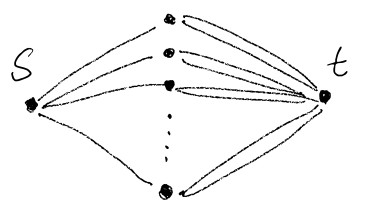
\includegraphics[width=0.4\linewidth]{figures/graph1.jpg}
\end{figure}

Removing any edge on the left side will increase the (s-t) min cut. 
Initially the left-side edges make up $\frac{1}{3}$ of the total amount of edges.
At every stage if the algorithm has not contracted any wrong edge, the probability of contracting a wrong edge is than at least $\frac{1}{3}$. Thus we see that the probability of obtaining the min-cut is at most

$$ \left(\frac{2}{3}\right)^{n-1} $$

Where $n$ is the total number of edges. (This is exponentially decreasing in $n$).

\subsection*{b}

Observe that any (s-t) min-cut define a unique split (2-partition) of the vertices.
To see this first note that an (s-t) min-cut defines a split of the vertices defined by whether they are connected with $s$ or not. 
Since it is a \emph{cut} it must have removed any edge between the two groups of vertices.
And since it is minimal, it cannot have removed any other edges. 
Thus it is unique.
Now the number of splits of $n$ vertices with $s$ in the first group and $t$ in the second is $2^{n-2}$.
So this is an upper bound on the number of min-cuts.
Consider the graph

\begin{figure}[H]
	\centering
	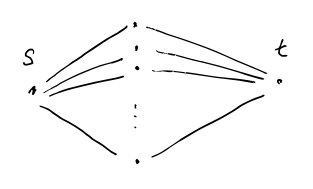
\includegraphics[width=0.4\linewidth]{figures/graph2.jpg}
\end{figure}

This achieves the upperbound of $2^{n-2}$ min-cuts, since any for any middle vertex you can choose either the left or the right edge to remove, resulting in a min-cut when done for all middle vertices.

\section*{Problem 2.1}

We claim that for any deterministic evaluation algorithm there is a $T_{d,k}$ tree which forces the algorithm to evaluate all subnodes (and leafs), and furthermore we can choose the root node to evaluate to $0$ and $1$ as we please.
Using DeMorgan it is easy to see that $d$-$\land$-$\lor$-trees are equivalent to $d$-$\downarrow$-trees so it is enough to consider these (we even allow the height to be odd).
We proceed by induction on the height $h$ of the tree. 
If $h = 0$ we are at leaf so we read $1 = d^0$ which we can choose to be $0$ or $1$.
If $h = n$ its subtrees are of lower height. 
By induction we can choose the first $d-1$ choices of subtrees of the algorithm to evaluate - using all nodes - to 0.
This is because each zero forces the algorithm to evaluate more subtrees.
The last chosen subtree of the algorithm we can choose to evaluate to $0$ or $1$ depending on whether we want the node to evaluate to $1$ resp. $0$.
This completes the argument.

\section*{Exercise 1.2}

Let $H_n$ be the \emph{hand weight graph} with $4n$ vertices, that is $2n$ on each side.
At any point if the algorithm chooses two vertices on different sides, we increase the min-cut.  After $n$ succesful steps (that is steps not resulting in larger min-cut) each side still has at least $n$ vertices left. The probability of choosing a pair from different sides during the first $n$ steps is at least

\begin{align*}
	\frac{\text{Number of pairs of vertices with each in different side}}
	{\text{Total number of pairs}}
	&\geq \frac{ n \cdot n }
	{4n \cdot (4n - 1) / 2}
	\\ &= \frac{n}{8n - 4}
	\\ &\geq \frac{1}{8}
\end{align*}

Thus the change of fail is a least $\left(\frac{7}{8}\right)^n$.
